\documentclass[11pt,a4paper]{article}

\usepackage[utf8]{inputenc}
\usepackage[margin=1in]{geometry}
\usepackage{amsmath,amssymb}
\usepackage{graphicx}
\usepackage{booktabs}
\usepackage{tabularx}
\usepackage{xcolor}
\usepackage{hyperref}
\usepackage{fancyhdr}
\usepackage{titlesec}
\usepackage{enumitem}
\usepackage{caption}
\usepackage{float}

% Colors
\definecolor{primaryblue}{RGB}{27, 54, 93}
\definecolor{accentgreen}{RGB}{13, 104, 50}
\definecolor{darkgray}{RGB}{60, 60, 60}
\definecolor{lightgray}{RGB}{245, 247, 250}
\definecolor{bordergray}{RGB}{210, 215, 225}

% Hyperref setup
\hypersetup{
    colorlinks=true,
    linkcolor=primaryblue,
    citecolor=primaryblue,
    urlcolor=primaryblue
}

% Header / Footer
\pagestyle{fancy}
\fancyhf{}
\lhead{\textcolor{primaryblue}{\textbf{AgriScan 360 --- Final Laboratory Report}}}
\rhead{\textcolor{darkgray}{CSE 4326: Micro Lab}}
\cfoot{\thepage}
\renewcommand{\headrulewidth}{0.6pt}

% Section Titles
\titleformat{\section}
  {\color{primaryblue}\normalfont\Large\bfseries}{\thesection}{1em}{}[\titlerule]
\titleformat{\subsection}
  {\color{primaryblue}\normalfont\large\bfseries}{\thesubsection}{1em}{}
\titleformat{\subsubsection}
  {\color{darkgray}\normalfont\normalsize\bfseries}{\thesubsubsection}{1em}{}

\begin{document}

% --- Title Page (UIU Micro Lab Official Cover Page) ---
\begin{titlepage}
    \centering
    \vspace*{0.2cm}
    
\includegraphics[width=3.6cm]{image1.jpeg}\\[0.5cm]
    {\LARGE \textbf{United International University}}\\[0.25cm]
    {\Large \textbf{Department of CSE}}\\[2.0cm]
    
    {\fontsize{32pt}{38pt}\selectfont \textbf{\color{primaryblue} AgriScan - 360}}\\[0.4cm]
    {\large \textbf{Automated Multi-Modal Non-Destructive Produce Quality, Internal Defect, and Freshness Inspection System}}\\[2.2cm]
    
    \begin{flushleft}
    \hspace{0.5cm}{\Large \textbf{Course Code: CSE 4326}}\\[0.3cm]
    \hspace{0.5cm}{\Large \textbf{Course Name: Microprocessors and Microcontrollers Laboratory}}\\[2.0cm]
    \end{flushleft}
    
    \begin{flushleft}
    \hspace{0.5cm}
    \setlength{\fboxsep}{12pt}
    \colorbox{lightgray}{%
    \begin{minipage}{0.88\textwidth}
        \textbf{\large Submitted by (Group no.): 02}\\[0.3cm]
        \textbf{\large Name: Md. Shafiul Bari}\\[0.3cm]
        \textbf{\large Student ID: 0112330837}
    \end{minipage}%
    }
    \end{flushleft}
    
    \vfill
    {\normalsize \textbf{Academic Session:} 2026 \quad $\vert$ \quad \textbf{Course:} CSE 4326 Microprocessors \& Microcontrollers Lab}
\end{titlepage}

\newpage
\tableofcontents
\newpage

% --- Section 1: Abstract & Introduction ---
\section{Abstract \& Introduction}

\subsection{Abstract}
Post-harvest food spoilage constitutes a critical economic and food-security crisis across developing agricultural economies such as Bangladesh, where an estimated 25\% to 40\% of harvested produce perishes prior to consumer distribution. Existing evaluation techniques in regional wholesale mandis remain either purely subjective (superficial human visual sorting that misses internal rot, hollow heart, and latent fungal pathogens) or destructively invasive (penetrometer punctures that ruin saleable produce). 

\textbf{AgriScan 360} resolves this trade-off by engineering an automated, multi-physics, non-destructive freshness inspection ecosystem for the CSE 4326 Microcontrollers Laboratory. The device integrates a gravity pipe feed chute gated by an SG90 micro-servo motor that drops produce into a 27-liter sealed dark chamber onto an 8-stop NEMA 17 stepper motor turntable ($45^\circ$ indexing). A Raspberry Pi 5 orchestrates simultaneous multi-modal sensing: continuous Volatile Organic Compound (VOC) headspace sniffing via a Bosch BME688 MOX gas sensor is executed in parallel with 16 synchronized optical captures (8 White-light RGB and 8 365 nm UV-A autofluorescence frames). Telemetry and multi-spectral imagery are streamed over HTTP multipart to a local host server running FastAPI and SQLite. A multi-modal decision engine fuses visual necrotic browning, fungal excitation, and dynamic gas resistance kinetics ($\Delta R$, drop ratio $\eta$, decay slope $dR/dt$) into a binary classification (\texttt{HEALTHY} vs. \texttt{ROTTEN}). Results are displayed locally on an SSD1306 OLED screen and on a live web dashboard. After scanning, the machine halts safely without automated sorting, allowing the human operator to manually pick up and sort the inspected item.

\subsection{Introduction}
Fresh fruits and vegetables are living biological tissues undergoing active metabolic respiration, transpiration, and volatile organic acid synthesis post-harvest. Traditional single-angle computer vision fails to detect early rot when decay occurs on the opposite side or internally near the seed cavity. Furthermore, latent fungal pathogens such as \textit{Botrytis cinerea} and \textit{Penicillium expansum} remain visually undetectable to the human eye for days before surface mycelium appears.

AgriScan 360 addresses these physical failure modes through three synchronized sensing pillars:
\begin{enumerate}[leftmargin=*]
    \item \textbf{Pillar 1: Complete $360^\circ$ Visible RGB Reflectance:} Captures 8 circumferential angles to eliminate visual blind spots, analyzing surface browning, skin integrity, and stem calyx condition.
    \item \textbf{Pillar 2: 365 nm UV-A Autofluorescence Excitation:} Stimulates fluorophores in fungal mycelium and leaked plant catabolites, revealing latent infections prior to visual spore emergence.
    \item \textbf{Pillar 3: Chemical Headspace E-Nose Kinetics:} Operates a Bosch BME688 MOX gas sensor in the sealed 27L enclosure, tracking VOC evaporation, fermentation ethanol, and respiration velocity.
\end{enumerate}

% --- Section 2: Objectives ---
\section{Project Objectives}
\begin{itemize}[leftmargin=*]
    \item \textbf{Comprehensive $360^\circ$ Spatial Assessment:} Eliminate visual occlusions by rotating produce across 8 discrete $45^\circ$ stops using a precision stepper-driven turntable.
    \item \textbf{Simultaneous Optical \& Chemical Acquisition:} Overlap dual-spectrum optical imaging (White RGB + 365 nm UV-A) with continuous chemical gas sniffing, reducing total testing time from ~5 minutes to ~3 minutes.
    \item \textbf{Automated Gravity Feed Mechanism:} Implement a pipe-loading flap door driven by an SG90 micro-servo ($180^\circ$ open, $90^\circ$ closed) that gently deposits produce onto the turntable center.
    \item \textbf{Calibrated Vision ROI Crop:} Isolate the fruit inside the concentric turntable ring ($X: 25\% - 76\%$, $Y: 41\% - 100\%$), cropping out background chamber walls and wiring for clean AI inference.
    \item \textbf{Robust Binary Freshness Classification:} Classify produce strictly into \texttt{HEALTHY} or \texttt{ROTTEN} categories, incorporating an automatic gas override rule for latent internal decay.
    \item \textbf{Affordable Hardware Budget:} Deliver the complete system under 25,000 BDT using commercial-off-the-shelf components sourced from Bangladesh suppliers (e.g., RoboticsBD.com).
\end{itemize}

% --- Section 3: Features ---
\section{Key System Features}
\begin{itemize}[leftmargin=*]
    \item \textbf{Inspect-and-Halt Workflow:} Follows an inspect-and-halt protocol without mechanical sorters or diverters. Produce is loaded via pipe, inspected across all modalities, and manually retrieved by the operator.
    \item \textbf{Dual Solid-State MOSFET Switching:} Two independent IRLZ44N logic-level MOSFETs switch the 12V White LED array and 365 nm UV-A LED array via 3.3V GPIO commands.
    \item \textbf{Dynamic Gas Kinetics Engine:} Continuously extracts baseline resistance $R_{\text{base}}$, minimum resistance $R_{\text{min}}$, net drop $\Delta R$, drop ratio $\eta$, and decay velocity slope $dR/dt$ using linear regression.
    \item \textbf{Internal Decay Gas Override:} If produce appears visually clean but headspace VOC drop exceeds thresholds ($\Delta R \ge 5.5\text{ k}\Omega$ or $\eta \ge 15\%$ for Tomato), the system automatically overrides vision and marks the produce \texttt{ROTTEN}.
    \item \textbf{Dual HMI Display:} Features an onboard SSD1306 OLED display for standalone operation and a real-time web dashboard broadcasting 16-frame image carousels and gas curves over WebSocket.
    \item \textbf{Live Telemetry Sync:} Automatically exports all completed scans and ground-truth labels from SQLite (\texttt{agriscan360.db}) to CSV (\texttt{bme688\_telemetry\_dataset.csv}) for ongoing machine learning model retraining.
\end{itemize}

% --- Section 4: Components ---
\section{Hardware Components Specification}
\begin{table}[H]
\centering
\small
\begin{tabularx}{\textwidth}{l p{4.5cm} X}
\toprule
\textbf{Component} & \textbf{Model / Specifications} & \textbf{Role in AgriScan 360} \\
\midrule
Raspberry Pi 5 (4GB) & Broadcom BCM2712 Quad Cortex-A76 @ 2.4GHz & Edge orchestrator, I2C master, GPIO controller, HTTP client \\
Pi Camera Module 2 & Sony IMX219 8.08MP, 1080p capture & Dual-spectrum RGB and UV-A optical imaging \\
BME688 MOX Sensor & Bosch Sensortec, I2C address 0x77 & Headspace VOC resistance, temperature, humidity, pressure \\
NEMA 17 Stepper & 17HS4401, 1.8$^\circ$ step, 40 N$\cdot$cm torque & 8-stop 360$^\circ$ turntable rotation \\
A4988 Motor Driver & Allegro Bipolar Microstepping Driver & Current-controlled drive for NEMA 17 stepper \\
SG90 Micro Servo & TowerPro 9g, 50 Hz PWM, 1.8 kg$\cdot$cm & Pipe feed chute entry door flap \\
SSD1306 OLED (0.96") & 128$\times$64 dot-matrix, I2C address 0x3C & Real-time local status and classification display \\
IRLZ44N MOSFETs (x2) & Logic-level N-Channel, $V_{GS(\text{th})} \le 2.0$V & 3.3V logic switching for 12V White and UV-A LEDs \\
365 nm UV-A LED Array & High-radiance 365 nm UV emitters & Latent fungal mycelium autofluorescence excitation \\
White LED Array & High-CRI diffused 12V LED array & Glare-free visible surface reflectance lighting \\
12V 2A DC SMPS & Regulated 12V 2A Power Adapter & Motor and LED illumination power rail \\
3.7V 18650 Battery & Li-ion cell with 5V boost circuit & Portable / backup logic supply \\
Test Chamber & 27-liter sealed dark box & Sealed atmosphere for headspace gas accumulation \\
\bottomrule
\end{tabularx}
\caption{Comprehensive Hardware Component Specifications}
\end{table}

% --- Section 5: Cost Analysis in BDT ---
\section{Cost Analysis in BDT (RoboticsBD Benchmark)}
Pricing verified against leading Bangladesh electronics suppliers, including \textbf{RoboticsBD.com} and local hardware vendors in Dhaka:

\begin{table}[H]
\centering
\begin{tabularx}{\textwidth}{l l X r r}
\toprule
\textbf{\#} & \textbf{Item Name} & \textbf{Source Reference} & \textbf{Unit Price (BDT)} & \textbf{Total (BDT)} \\
\midrule
1 & Raspberry Pi 5 (4GB RAM) & RoboticsBD / TechshopBD & 15,500 & 15,500 \\
2 & Raspberry Pi Camera Module 2 (IMX219) & RoboticsBD.com & 2,450 & 2,450 \\
3 & NEMA 17 Stepper Motor (17HS4401) & RoboticsBD.com & 1,250 & 1,250 \\
4 & A4988 Stepper Motor Driver Module & RoboticsBD.com & 140 & 140 \\
5 & TowerPro SG90 9g Micro Servo & RoboticsBD.com & 140 & 140 \\
6 & Bosch BME688 Gas Sensor Module & RoboticsBD.com & 1,850 & 1,850 \\
7 & SSD1306 0.96" I2C OLED Display & RoboticsBD.com & 320 & 320 \\
8 & 365 nm High-Power UV-A LED Array & RoboticsBD / Local Market & 450 & 450 \\
9 & High-CRI White Diffused LED Strip & Local Market & 220 & 220 \\
10 & Dual IRLZ44N MOSFET Board & Local Market & 180 & 180 \\
11 & 12V 2A DC Power Adapter (SMPS) & RoboticsBD.com & 420 & 420 \\
12 & 3.7V 18650 Battery + Holder & RoboticsBD.com & 320 & 320 \\
13 & 27L Chamber Box, Pipe, Acrylic Turntable & Local Fabrication & 1,400 & 1,400 \\
14 & Jumpers, Perfboard, Fasteners & Local Market & 350 & 350 \\
\midrule
\textbf{Total} & \multicolumn{3}{l}{\textbf{Complete Multi-Modal AgriScan 360 System}} & \textbf{24,990 BDT} \\
\bottomrule
\end{tabularx}
\caption{Itemized Bill of Materials (BOM) in Bangladeshi Taka (BDT)}
\end{table}

\noindent\textbf{Economic Viability:} Commercial single-modal fruit inspection and sorting machines (e.g., Tomra, Compac, Aweta) range from \$35,000 to \$120,000 USD (>40,00,000 BDT). AgriScan 360 delivers an automated multi-spectral optical and chemical inspection platform for \textbf{under 25,000 BDT} ($\approx \$210$ USD), representing a 99\% cost reduction.

% --- Section 6: Circuit Diagram & Pin Mapping ---
\section{Circuit Diagram \& Hardware Interconnections}

\begin{figure}[H]
\centering
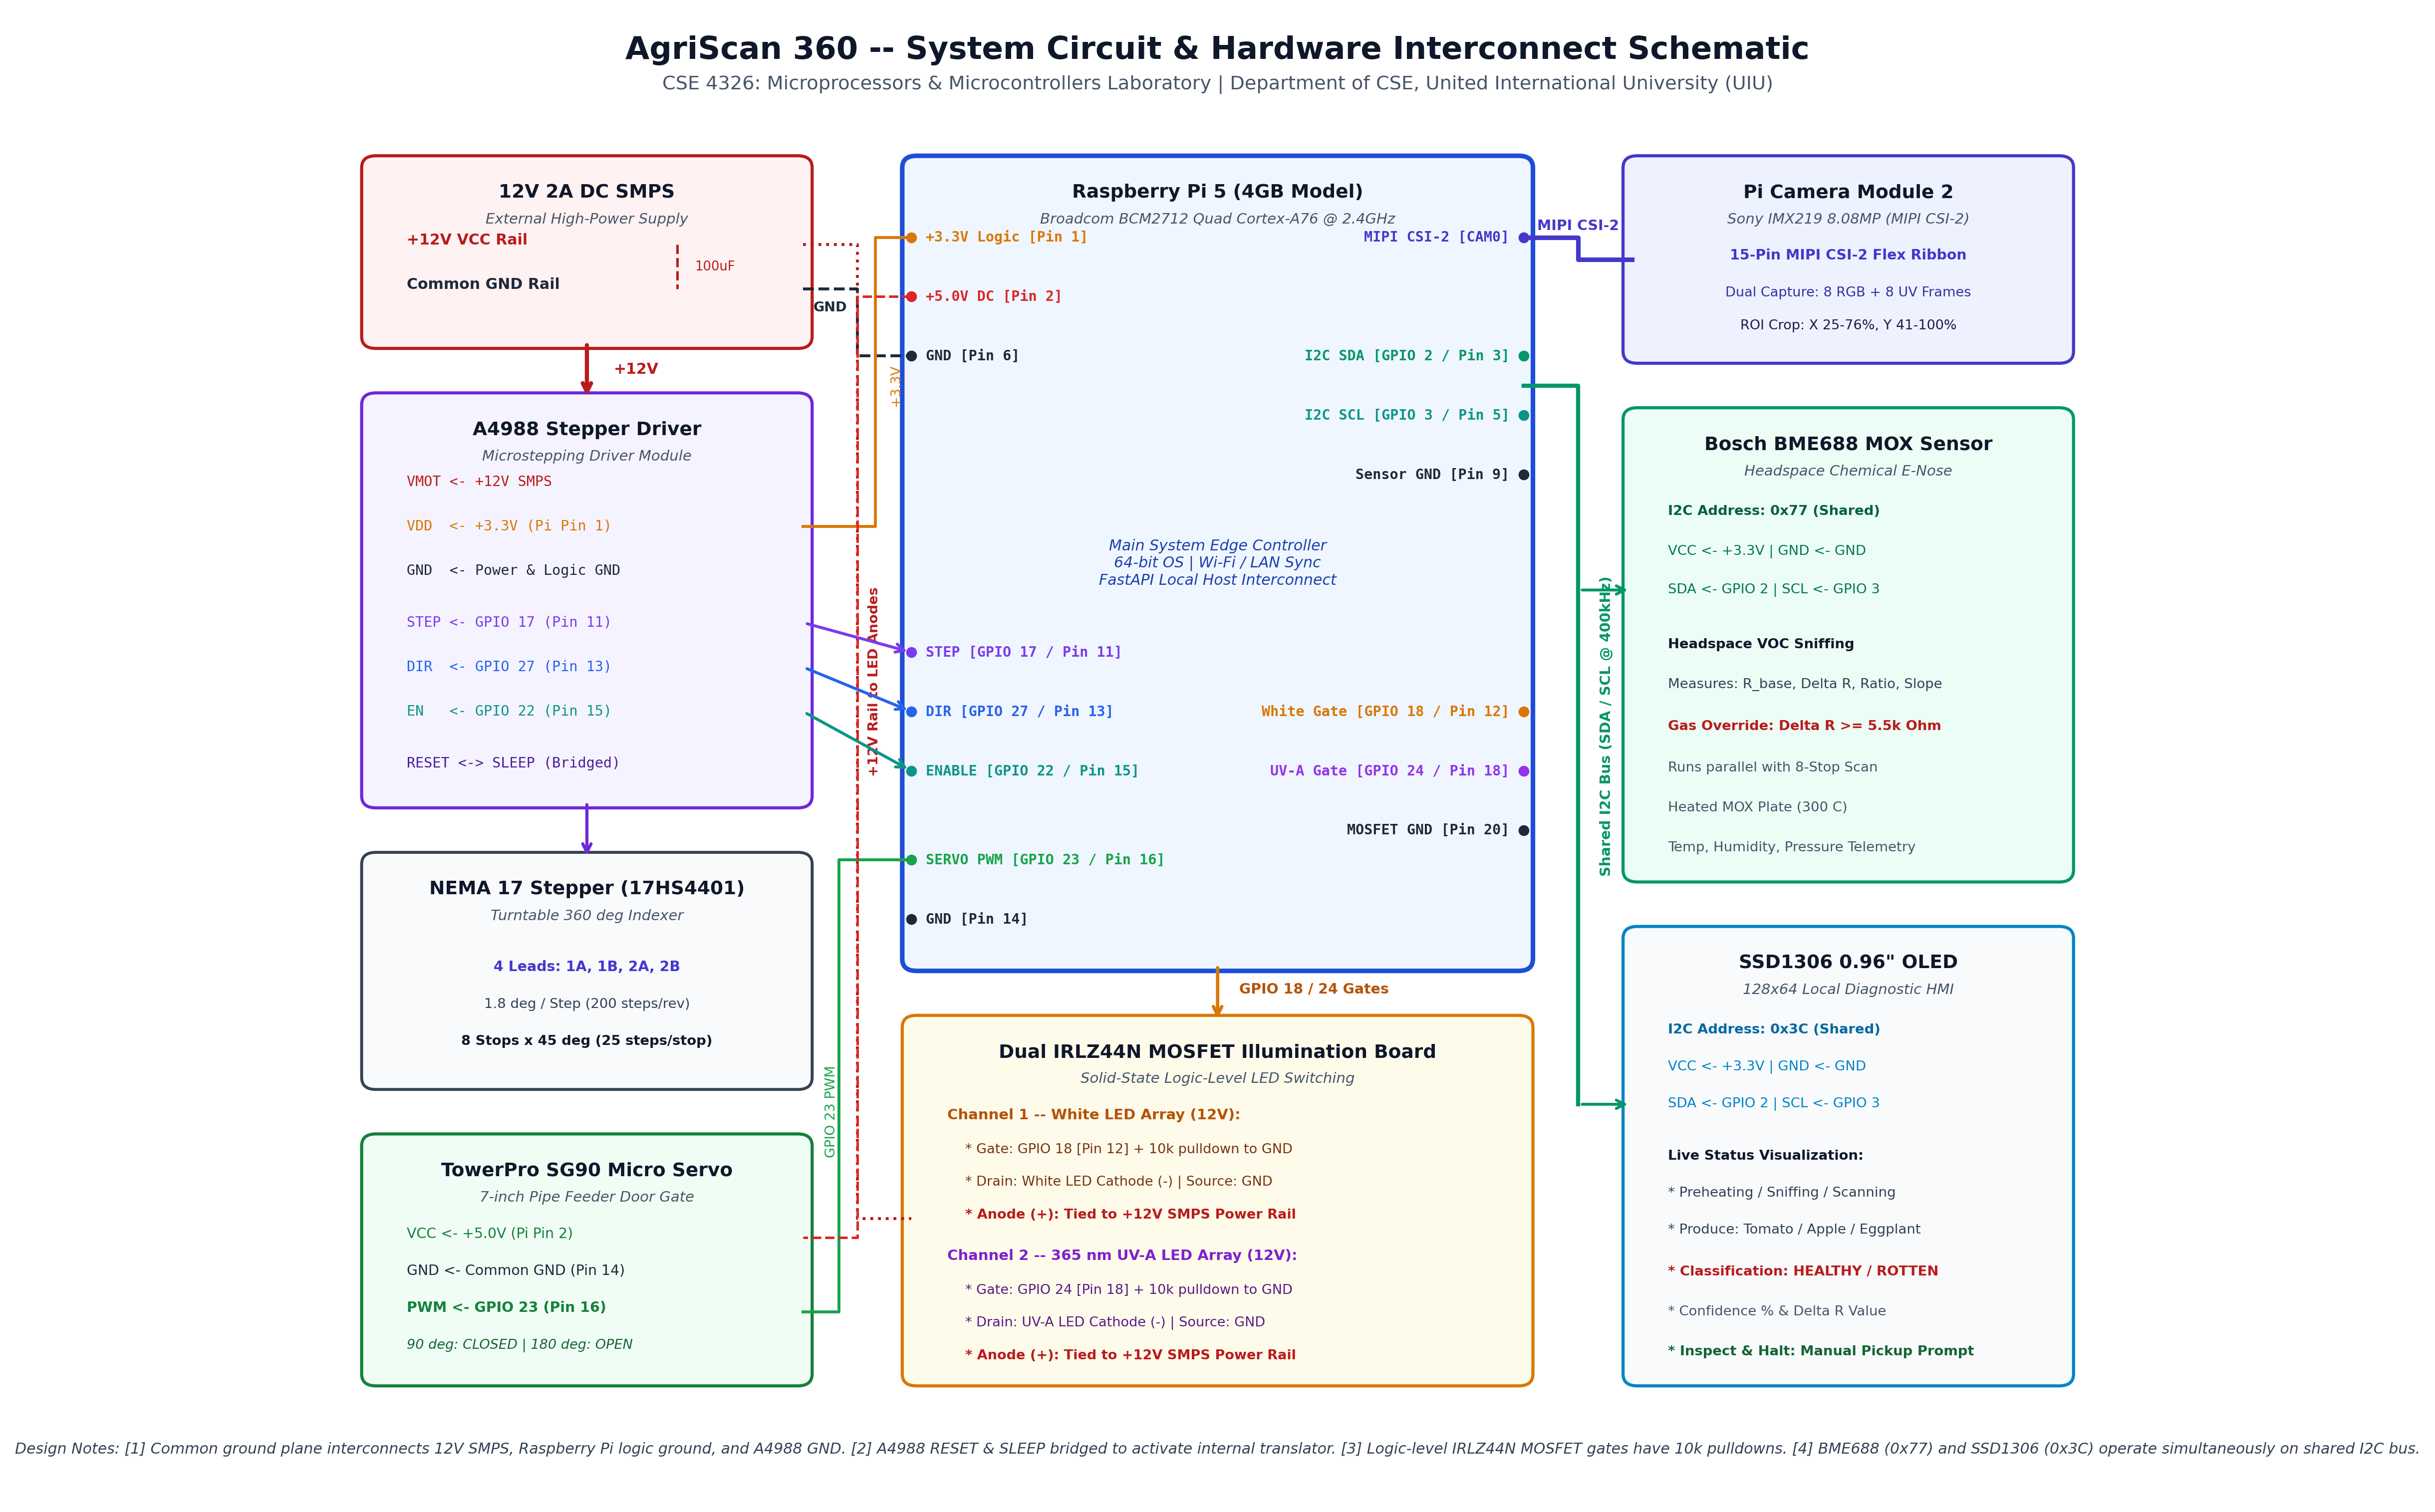
\includegraphics[width=\textwidth]{circuit_diagram.png}
\caption{Complete AgriScan 360 System Circuit Schematic and Interconnect Architecture}
\label{fig:circuit_diagram}
\end{figure}

\noindent\textbf{Circuit Architecture \& Power Distribution:}
The complete electrical interconnect architecture is orchestrated by the Raspberry Pi 5 acting as edge master. To prevent electrical noise and ground bounce from inductive loads, a dual-rail power scheme is enforced:
\begin{enumerate}[leftmargin=*]
    \item \textbf{External 12V 2A SMPS Rail:} Powers the NEMA 17 stepper motor through the A4988 driver VMOT pin, decoupled with a $100\ \mu\text{F}$ 25V electrolytic capacitor. This same rail supplies the White and 365 nm UV-A LED arrays.
    \item \textbf{Logic Power \& Isolation:} The Raspberry Pi provides 3.3V logic reference to A4988 VDD and sensor pullups, and 5.0V DC to the SG90 micro-servo motor. All power returns meet at a star common ground plane.
    \item \textbf{Solid-State Switching:} High-power illumination switching is executed by dual IRLZ44N logic-level N-channel MOSFETs with $10\text{ k}\Omega$ pulldown resistors at their gates, ensuring reliable 3.3V GPIO switching without gate float.
    \item \textbf{Shared I2C Bus:} The Bosch BME688 MOX sensor (address \texttt{0x77}) and SSD1306 OLED display (address \texttt{0x3C}) communicate simultaneously over I2C1 (GPIO 2 SDA, GPIO 3 SCL) at 400 kHz.
\end{enumerate}

\newpage
\subsection{Raspberry Pi 5 Pin Mapping}
\begin{table}[H]
\centering
\small
\begin{tabularx}{\textwidth}{l l l l}
\toprule
\textbf{Component Pin} & \textbf{Raspberry Pi 5 Pin} & \textbf{Signal Type} & \textbf{Electrical Specification} \\
\midrule
A4988 STEP & GPIO 17 (Physical Pin 11) & Digital Output & 3.3V pulse ($5\text{ ms}$ width) \\
A4988 DIR & GPIO 27 (Physical Pin 13) & Digital Output & HIGH = CW, LOW = CCW \\
A4988 ENABLE & GPIO 22 (Physical Pin 15) & Digital Output & Active-LOW: LOW = Motor ON, HIGH = Motor OFF \\
A4988 VMOT / GND & 12V 2A SMPS Rail & Motor Power & 12V DC with $100\ \mu\text{F}$ capacitor \\
A4988 VDD / GND & 3.3V (Pin 1) / GND (Pin 6) & Logic Power & 3.3V logic reference \\
SG90 Servo PWM & GPIO 23 (Physical Pin 16) & Hardware PWM & 50 Hz PWM ($90^\circ$ closed, $180^\circ$ open) \\
SG90 VCC / GND & 5V Rail (Pin 2) / GND (Pin 14) & Servo Power & 5V DC supply \\
White MOSFET Gate & GPIO 18 (Physical Pin 12) & Digital Output & 3.3V logic with $10\text{ k}\Omega$ pulldown \\
UV-A MOSFET Gate & GPIO 24 (Physical Pin 18) & Digital Output & 3.3V logic with $10\text{ k}\Omega$ pulldown \\
BME688 SDA & GPIO 2 (Physical Pin 3) & I2C Data & Shared I2C bus, address 0x77 \\
BME688 SCL & GPIO 3 (Physical Pin 5) & I2C Clock & Shared I2C bus \\
SSD1306 SDA & GPIO 2 (Physical Pin 3) & I2C Data & Shared I2C bus, address 0x3C \\
SSD1306 SCL & GPIO 3 (Physical Pin 5) & I2C Clock & Shared I2C bus \\
Pi Camera v2 & CAM0 / CAM1 Port & MIPI CSI-2 & 15-pin serial camera ribbon \\
\bottomrule
\end{tabularx}
\caption{Complete Raspberry Pi 5 Hardware Interconnect Pin Mapping}
\end{table}

% --- Section 7: Working Principle & Implementation ---
\section{Working Principle \& Implementation}

\subsection{Operational Protocol (Inspect-and-Halt Workflow)}
\begin{enumerate}[leftmargin=*]
    \item \textbf{Step A --- Clean-Air Baseline Sniffing:} The empty 27L chamber is closed. The BME688 pre-heats and sniffs for 180 seconds. The first 120 seconds are discarded for thermal stabilization; the final 5 seconds establish the reference baseline resistance $R_{\text{base}}$.
    \item \textbf{Step B --- Pipe Drop \& Auto-Detection:} The operator drops produce into the top pipe. The SG90 servo opens to $180^\circ$ for 2 seconds, releasing the fruit onto the turntable, and closes to $90^\circ$. The lid is secured. The camera captures a test image with ROI cropping ($X: 25\% - 76\%$, $Y: 41\% - 100\%$) and classifies the fruit type (Tomato, Apple, or Eggplant) via HSV color space analysis.
    \item \textbf{Step C --- Simultaneous Sniffing \& 8-Stop Scan:} Continuous BME688 sniffing launches on a background thread. Simultaneously, the NEMA 17 motor steps through 8 angular positions ($45^\circ$ each). At each stop:
    \begin{itemize}
        \item White LED activates $\to$ captures RGB frame $\to$ LED turns off.
        \item UV-A LED activates $\to$ captures UV fluorescence frame $\to$ LED turns off.
        \item Turntable advances 25 steps ($45^\circ$).
    \end{itemize}
    All 16 photos finish in ~100 seconds. If incubation time remains, the system counts down the remaining seconds (skippable via Ctrl+C).
    \item \textbf{Step D --- Decision Fusion \& Result Display:} The Pi stops gas sniffing, compiles $\Delta R$, $\eta$, and decay slope $dR/dt$, and uploads all 16 frames + gas telemetry to the FastAPI server. The AI classifies the sample:
    \begin{equation}
        \text{Fused Score} = 0.40 \cdot P_1 + 0.35 \cdot P_2 + 0.25 \cdot P_3
    \end{equation}
    If $\text{Fused Score} \ge 0.40$ or $P_3 \ge 0.70$ (gas override), status is \texttt{ROTTEN}; otherwise \texttt{HEALTHY}.
    \item \textbf{Step E --- Manual Pickup (No Sorting Mechanism):} The status is shown on the OLED display and web UI. Motor coils de-energize. \textbf{The machine halts completely.} The operator manually opens the lid, removes the fruit, and sorts it based on the displayed result.
\end{enumerate}

% --- Section 8: Results & Applications ---
\section{Results \& Applications}

\subsection{Experimental Scan Records}
\begin{table}[H]
\centering
\small
\begin{tabularx}{\textwidth}{c l c r r r r l c}
\toprule
\textbf{ID} & \textbf{Produce} & \textbf{Ground Truth} & \textbf{$R_{\text{base}}$} & \textbf{$R_{\text{post}}$} & \textbf{$\Delta R$} & \textbf{Ratio $\eta$} & \textbf{AI Result} & \textbf{Confidence} \\
\midrule
08 & Tomato & \textbf{HEALTHY} & 270.66 k$\Omega$ & 267.02 k$\Omega$ & 3.64 k$\Omega$ & 2.26\% & \textbf{HEALTHY} & 88.2\% \\
11 & Tomato & \textbf{ROTTEN} & 263.15 k$\Omega$ & 212.98 k$\Omega$ & 50.17 k$\Omega$ & 19.65\% & \textbf{ROTTEN} & 94.0\% \\
13 & Tomato & \textbf{ROTTEN} & 259.66 k$\Omega$ & 251.72 k$\Omega$ & 7.94 k$\Omega$ & 4.21\% & \textbf{ROTTEN} & 78.5\% \\
14 & Tomato & \textbf{HEALTHY} & 268.38 k$\Omega$ & 262.99 k$\Omega$ & 5.39 k$\Omega$ & 4.47\% & \textbf{HEALTHY} & 87.5\% \\
\bottomrule
\end{tabularx}
\caption{Empirical Experimental Telemetry from Real Chamber Scans}
\end{table}

\subsection{Practical Applications}
\begin{itemize}[leftmargin=*]
    \item \textbf{Wholesale Market Intake:} Rapid testing of incoming crates to isolate batches with early fungal decay before distribution.
    \item \textbf{Cold Storage Screening:} Pre-entry screening to avoid storing fruits with latent fungal rot that emit ethylene and spoil adjacent produce.
    \item \textbf{Quality Control in Packhouses:} Non-destructive validation of premium export produce.
\end{itemize}

% --- Section 9: Social Impact & Future Scope ---
\section{Social Impact \& Future Scope}

\subsection{Social Impact in Bangladesh}
\begin{itemize}[leftmargin=*]
    \item \textbf{Reducing Post-Harvest Waste:} Preserves marketable volumes of high-value perishables (tomatoes, eggplants) without additional fertilizer or water use.
    \item \textbf{Empowering Smallholder Farmers:} Provides an objective, low-cost freshness evaluation to prevent unfair price discounts from middlemen.
    \item \textbf{Public Health Protection:} Identifies fungal mycotoxins (e.g., patulin from \textit{Penicillium}) before produce enters local markets.
\end{itemize}

\subsection{Future Scope}
\begin{itemize}[leftmargin=*]
    \item \textbf{Automated Diverter Arm:} Add a dual-bin servo diverter to sort items into \texttt{HEALTHY} and \texttt{REJECT} bins automatically, eliminating manual pickup.
    \item \textbf{Conveyor Integration:} Replace the turntable with an indexed roller conveyor to increase throughput from ~20 to >600 items/hour.
    \item \textbf{Vis-NIR Spectroscopy:} Integrate an AS7265x multi-spectral sensor ($410 - 940$ nm) for non-destructive sugar content ($^\circ\text{Brix}$) and internal moisture measurement.
    \item \textbf{Standalone Edge NPU:} Quantize models to INT8 to run entirely on the Raspberry Pi 5 using a Hailo-8L NPU accelerator, removing the need for an external laptop server.
\end{itemize}

% --- Section 10: Conclusion & References ---
\section{Conclusion \& References}

\subsection{Conclusion}
AgriScan 360 demonstrates that multi-modal sensing combining 360$^\circ$ optical imaging, UV-A autofluorescence, and dynamic metal-oxide headspace kinetics provides reliable, non-destructive produce freshness evaluation. Running 16-photo image capture simultaneously with continuous BME688 sniffing delivers complete inspections within ~3 minutes. With an inspect-and-halt protocol and manual retrieval, the system achieves commercial-grade evaluation at a bill-of-materials cost under 25,000 BDT, providing a practical, accessible solution for post-harvest quality assessment in developing agricultural economies.

\subsection{References}
\begin{enumerate}[leftmargin=*]
    \item Sanz, V. et al. (2018). \textit{Quality evaluation of fresh produce using electronic nose technology}. Postharvest Biology and Technology, 142, pp. 88--96.
    \item Lorente, D. et al. (2012). \textit{Recent advances and applications of hyperspectral imaging for fruit and vegetable quality assessment}. Food and Bioprocess Technology, 5(4), pp. 1121--1142.
    \item Moshou, D. et al. (2005). \textit{Plant disease detection using spectral reflectance and UV-induced fluorescence}. Biosystems Engineering, 90(4), pp. 431--440.
    \item Bosch Sensortec (2021). \textit{BME688 Low Power Gas, Pressure, Temperature \& Humidity Sensor with AI}. Data Sheet BST-BME688-DS000-01.
    \item Kader, A. A. (2002). \textit{Postharvest Technology of Horticultural Crops}. University of California Agriculture and Natural Resources, Publication 3311.
    \item Bari, M. S. (2026). \textit{AgriScan 360 Dataset: Multi-Modal Optical and E-Nose Headspace Kinetics for Produce Freshness Evaluation}. Hugging Face Dataset Repository.
\end{enumerate}

\end{document}
